%% 
%% Copyright 2007-2025 Elsevier Ltd
%% 
%% This file is part of the 'Elsarticle Bundle'.
%% ---------------------------------------------
%% 
%% It may be distributed under the conditions of the LaTeX Project Public
%% License, either version 1.3 of this license or (at your option) any
%% later version.  The latest version of this license is in
%%    http://www.latex-project.org/lppl.txt
%% and version 1.3 or later is part of all distributions of LaTeX
%% version 1999/12/01 or later.
%% 
%% The list of all files belonging to the 'Elsarticle Bundle' is
%% given in the file `manifest.txt'.
%% 
%% Template article for Elsevier's document class `elsarticle'
%% with harvard style bibliographic references

\documentclass[preprint,12pt,authoryear]{elsarticle}

%% Use the option review to obtain double line spacing
%% \documentclass[authoryear,preprint,review,12pt]{elsarticle}

%% Use the options 1p,twocolumn; 3p; 3p,twocolumn; 5p; or 5p,twocolumn
%% for a journal layout:
%% \documentclass[final,1p,times,authoryear]{elsarticle}
%% \documentclass[final,1p,times,twocolumn,authoryear]{elsarticle}
%% \documentclass[final,3p,times,authoryear]{elsarticle}
%% \documentclass[final,3p,times,twocolumn,authoryear]{elsarticle}
%% \documentclass[final,5p,times,authoryear]{elsarticle}
%% \documentclass[final,5p,times,twocolumn,authoryear]{elsarticle}

%% For including figures, graphicx.sty has been loaded in
%% elsarticle.cls. If you prefer to use the old commands
%% please give \usepackage{epsfig}

%% The amssymb package provides various useful mathematical symbols
\usepackage{amssymb}
%% The amsmath package provides various useful equation environments.
\usepackage{amsmath}
%% The amsthm package provides extended theorem environments
%% \usepackage{amsthm}

%% The lineno packages adds line numbers. Start line numbering with
%% \begin{linenumbers}, end it with \end{linenumbers}. Or switch it on
%% for the whole article with \linenumbers.
\usepackage{lineno}

\usepackage{tabularx}
\usepackage{booktabs}

\journal{Nuclear Physics B}




\begin{document}
\linenumbers
\begin{frontmatter}

%% Title, authors and addresses

%% use the tnoteref command within \title for footnotes;
%% use the tnotetext command for theassociated footnote;
%% use the fnref command within \author or \affiliation for footnotes;
%% use the fntext command for theassociated footnote;
%% use the corref command within \author for corresponding author footnotes;
%% use the cortext command for theassociated footnote;
%% use the ead command for the email address,
%% and the form \ead[url] for the home page:
%% \title{Title\tnoteref{label1}}
%% \tnotetext[label1]{}
%% \author{Name\corref{cor1}\fnref{label2}}
%% \ead{email address}
%% \ead[url]{home page}
%% \fntext[label2]{}
%% \cortext[cor1]{}
%% \affiliation{organization={},
%%            addressline={}, 
%%            city={},
%%            postcode={}, 
%%            state={},
%%            country={}}
%% \fntext[label3]{}

\title{Conditioning co-operation with property rights in a tragedy of the commons setting} %% Article title

%% use optional labels to link authors explicitly to addresses:
\author[label1]{Jakub Bandurski\corref{cor1}}
\cortext[cor1]{Corresponding author}
\ead{j.bandurski@uw.edu.pl}
\affiliation[label1]{organization={University of Warsaw, Faculty of Economic Sciences},
            addressline={Długa street 44/50},
            city={Warsaw},
            postcode={00-241},
            % state={},
            country={Poland}}



\author[label1]{Piotr Wójcik}
\ead{ pwojcik@wne.uw.edu.pl}

% \affiliation[label2]{organization={},
%             addressline={},
%             city={},
%             postcode={},
%             state={},
%             country={}}

% \author{} %% Author name

%% Author affiliation
% \affiliation{organization={},%Department and Organization
%             addressline={}, 
%             city={},
%             postcode={}, 
%             state={},
%             country={}}

%% Abstract
\begin{abstract}
%% Text of abstract
This article investigates the impact of property rights as external motivators behind the emergence of co-operative behaviour between Multi-agent Reinforcement Learning agents in a tragedy of the commons setting. Training and evaluation environments are specifically designed to incorporate collective and private property rights. The agents are evaluated in homogeneous and heterogeneous scenarios. Conclusions are drawn based on statistical analysis of the results, and behaviours are examined on the basis of videos generated. The results indicate that agents trained in a collective environment are more likely to co-operate, while agents trained in a private environment display more selfish behaviour. A basis is provided for further research into the external motivators influencing the emergence of co-operation between MARL agents in various socio-economic settings.
\end{abstract}
%%Graphical abstract
% \begin{graphicalabstract}
%\includegraphics{grabs}
% \end{graphicalabstract}

%%Research highlights
\begin{highlights}
\item First study to test property rights as external motivators in MARL cooperation
\item Novel design of environments modeling private vs. collective property regimes
\item Collective property agents show significantly higher cooperation levels 
\item Bimodal score distributions reveal diversity in cooperative strategies
\item Practical implications for sustainable AI systems in socio-economic applications

\end{highlights}

%% Keywords
\begin{keyword}
%% keywords here, in the form: keyword \sep keyword
Multi-agent Reinforcement Learning \sep cooperation \sep tragedy of commons \sep property rights
%% PACS codes here, in the form: \PACS code \sep code

%% MSC codes here, in the form: \MSC code \sep code
%% or \MSC[2008] code \sep code (2000 is the default)

\end{keyword}

\end{frontmatter}
%%%%%%%%%%%%%%%%%%%%%%%%%%%%%%%%%%%%%%%%%%%%%%%%%%%%%%%%%%%%%%%%%%%%%%%%

\section{Introduction}

The ability to co-operate is one of the most essential elements of a successful society. People are naturally social beings, they have ever been evolving complex mechanisms that allow them to work together effectively. This ability has enabled humans to build advanced civilizations, create innovative technologies, and address challenges that no individual could face alone. At the same time, co-operation carries inherent risks, as when individuals act selfishly, exploiting the willingness of others to work together. A textbook example of such a situation is the tragedy of the commons described by~\cite{hardin1968tragedy}. 

Given the importance of co-operation between people, it has now become even more essential to ensure that these behavioural patterns are understood and executed by the Artificial Intelligence agents being developed. A broad overview of the necessary moral guidance in creating AI agents has been covered by ~\cite{Bostrom2018}. If considerations like theirs are omitted in the future progression of AI in its direct interactions with people, AI may conceivably cause more harm than benefit to society.

Multi-agent Reinforcement Learning (MARL) has emerged as a powerful tool for studying and modelling socio-economic settings, thereby offering a way to create specific environments and test how agents interact with one another within them. Because real-world settings most often require interaction between multiple agents, MARL stands as the state-of-the-art framework for researching these topics. Significant progress in this field has been initiated by the publication of the open-source Melting Pot library \citep{Leibo2021, agapiou2023meltingpot20} which has implemented over thirty socio-economic scenarios suitable for MARL experiments.

When it comes to influencing the behaviour of MARL agents in socio-economic settings, this is usually done in reliance on reward function augmentations, as in \cite{Willis2023a}, \cite{Willis2023b}, \cite{Peysakhovich2017}, and \cite{Hughes2018}. Such studies commonly cover solely internal motivators, foregoing external ones. The impact of different property rights on co-operation and economic growth have led us to question whether property rights as an external motivator can impact the development of co-operative behaviour. The results are varied with both collective property rights and private property rights having positive impacts in various real-world socio-economic settings \citep{anderson2003property, Ostrom1990, Jaffe1996, Haydarolu2015, Baragwanath2023, montero2022cooperative}. Thus, our article investigates three research hypotheses. In the first we state that the agents trained in an environment with collective property rights will be more prone to co-operate than agents trained in environments with private property rights. The second one assumes that the agents trained in collective property environments will achieve higher “well-being”, on average, than those trained in private property environments. Lastly, the third hypothesis assumes that the inclusion of agents trained in collective property environments into a population will increase the average “well-being” of the population.

Previous works in this field focus on the augmentations of reward functions with intrinsic motivators. The innovation of our study stems from the realization that internal motivators, while crucial, are not the sole drivers of co-operation and that the impact of external motivators should be researched. The external motivator proposed and studied in this article is that of property rights.

Through investigating the behaviour of MARL agents trained in environments with different property rights, this study aims to contribute to a better understanding of how external factors can influence the development of co-operative behaviours. The findings have implications for the design of real-world systems involving resource management, where promoting co-operation is essential for sustainable and equitable outcomes.

The structure of this article is as follows. Section 1 reviews the literature regarding related works on emerging co-operation and the incorporation of Multi-agent Reinforcement Learning into socio-economic settings. In Section 2 the MARL methodology used for the purpose of the study is closely outlined. The analytical framework including the design of the training and evaluation environments and model implementation is covered in Section 3. Finally, Section 4 provides the results of the simulations and their statistical analysis. Evaluation scenarios are extensively described and compared. The behaviour of the agents is observed based on generated videos. The last section summarizes the key conclusions of this article.

%%%%%%%%%%%%%%%%%%%%%%%%%%%%%%%%%%%%%%%%%%%%%%%%%%%%%%%%%%%%%%%%%%%%%%%%

\section{Background}

\subsection{Multi-agent Reinforcement Learning in socio-economic settings}

Multi-agent Reinforcement Learning, can be used to explore and research game theory, microeconomics, and even socio-economic dilemmas. Having the ability to design environments, possible actions, reward functions, and the possibility to propose numerous learning approaches, is very useful in understanding socio-economic settings without the necessity of studying the behaviour of groups of people. A team of researchers from DeepMind created a framework of more than 30 games that can be used for researching the cross-section of fields of MARL and socio-economic dilemmas \citep{Leibo2021, agapiou2023meltingpot20}. The main purpose of the Melting Pot framework is to provide tools for evaluating MARL algorithms in scenarios unforeseen in the training process. In one of the papers using Melting Pot, the authors performed studies on environmental features needed for agents to develop microeconomic phenomena such as trade, specialization, and utility maximization  \citep{Johanson2022}. The framework has been used in a study of co-operation in mixed settings where the self-interest of the agents worsens results for the entire group in the long term, similar to the tragedy of the commons. The authors propose the minimal reward transfer as a metric of the difference between the agent’s optimum and the groups’ optimum \citep{Willis2023a, Willis2023b}. The minimal reward transfer is the smallest fraction of reward that needs to be transferred to other agents for the emergence of co-operation in a group. The paper showed that reward transfer can be utilized to modify settings so that co-operation becomes the rational choice of each agent, whereas the same scenarios without reward sharing suffer from the tragedy of the commons. Another common approach is to relate the intrinsic reward augmentation with the mean reward of all agents. It has been shown that for cases where the relation is positive, the MARL agents can converge their behaviour to better equilibrium in socio-economic settings see \citep{Peysakhovich2017}. When the relation between the mean reward of the population and individual reward is negative it can shape behaviour efficiently, especially in settings where punishment mechanisms are present. Agents’ rewards are decreased when at least one agent is getting much lower results, and this in turn promotes non-discriminatory behaviour see \cite{Hughes2018}.

Previous works in this field focus on the augmentations of reward functions with intrinsic motivators see \citep{Peysakhovich2017, Perolat2017, Hughes2018, Willis2023a, Willis2023b}. However, they do not explore the impacts of external motivators such as altered training environments resembling social conventions. Augmenting the training process without changes to the agents’ architecture or reward functions could lead to faster and more cost-effective learning paths toward social norms and co-operation. Therefore, we propose specifically designed training environments inspired by property rights to ensure co-operation among MARL agents. Agents trained in two separate populations (one with the implementation of private property and a second one with collective property incorporated into the training environment) are later evaluated in a tragedy of the commons setting. The more effective the co-operation, the better the results achieved as a population in this scenario, therefore it is a proxy measure for the process of the emergence of co-operation.
 
The literature review lead us to ask whether the type of property rights could be a significant factor in the emergence of co-operation between agents in socio-economic settings. Further, is it possible to reduce or remove unwanted selfish behaviours through the design of appropriate training environments? 

% \subsection{Game Theory perspective}

% In the original work \cite{hardin1968tragedy}  outlined the tragedy of the commons with an example of publicly available pasture. Each of the herdsmen can choose how many of their cows will be kept on the pasture. The gains of every agent are proportional to the size of their herd. Given that the herdsmen are behaving rationally i.e. maximizing their individual gains they are faced with the following line of thought. The utility gain from adding one more cow to the pasture needs to be assessed. The direct benefit of increasing the cattle size by $1$ is received solely by the herdsman, whereas the cost being the exhaustion of the common pasture is split among all the agents. In turn, the author concludes, that the utility of adding a new animal to the herd is always positive. From here the tragedy can be seen as all of the agents are coming to the same conclusions and all of them increase the cattle size without limit, while the common resource is limited. The Nash equilibrium strategy profile proves to be the defect for all agents involved in the setting.

% From another perspective, the Pareto optimal strategy in the tragedy of the commons involves resource use that maximizes collective welfare, ensuring that no individual can be made better off without making someone else worse off. This outcome typically requires co-operation among agents to regulate consumption and maintain the sustainability of resources. Pareto optimality is achieved when the aggregate benefits of resource use are distributed in a way that avoids depletion while ensuring fairness among users. In essence, the Pareto optimal strategy profile is for all agents to co-operate and not deplete the common resource above a certain threshold. However, achieving Pareto optimality is inherently challenging due to the risk of free-riding and the difficulty of enforcing agreements in the absence of strong institutions or trust among users \cite{Ostrom1990}.

% The literature indicated that in non-cooperative settings with common resources, rational agents will select the best individual strategies that will not reach Pareto optimal outcomes. In turn, the decisions that are rational in the individual context lead to outcomes that are not rational in the social context see \citep{Maldonado2016}. The renewable resource model as in \cite{clark1974mathematical} can be used to show the divergence between the optimal management of the resource and the depletion caused by self-interested agents. It is noteworthy that the temporal dynamics of the tragedy of the commons are not usually taken into account as underlined in \cite{brekke2007effect}. Therefore the task of predicting agents’ behaviour becomes more cumbersome in empirical studies.

\subsection{Co-operation motivators in socio-economic settings}

One of the cornerstones of humanity’s success in developing a worldwide civilization is the ability to co-operate with others. Co-operation was a significant factor that allowed early humans to survive at all, and then to advance technologically and culturally. As societies evolved, so did co-operative mechanisms, taking shape in various forms such as trade networks, alliances, and social norms. Understanding the relevant dynamics can provide insights into how societies can address challenges and mitigate conflicts.

Co-operation, while beneficial in most settings, can also pose inherent risks of selfish behaviours and exploitation by individuals. A well-established problem in the field of economics of this nature is known as the tragedy of the commons. The tragedy of the commons refers to situations where individuals, acting in self-interest, deplete or harm a shared resource, ultimately leading to its loss. This problem was described by \cite{hardin1968tragedy} with an example of a common pasture where multiple farmers keep their livestock. From the perspective of each individual farmer, the best strategy is to maximize the size of their livestock. However, when everyone starts implementing this strategy, the pasture becomes overgrazed, and this causes long-term damage to the ecosystem and society. The solution would be to co-operate and optimize the size of livestock within the constraints of sustainable resource management.

To address these challenges, multiple strategies and mechanisms have been proposed. Some researchers argue that property rights are a crucial factor in defining and establishing effective co-operation. In \cite{anderson2003property} authors discuss how clearly defined private property rights can incentivize individuals to take responsibility for common resources and develop them sustainably. Property rights are a key component of the well-known principles of governing common resources set by \cite{Ostrom1990}. In general economics research, private property rights have been linked multiple times to the economic growth of countries. In \cite{Jaffe1996} authors conclude that powerful property rights are related to higher incentives to be more efficient with resources, therefore leading to elevated economic efficiency. A later study on OECD and EU markets showed similar results – namely, that a stronger institutional structure of property rights positively impacts economic growth \citep{Haydarolu2015}. On the other hand, some scholars find that the implementation of collective property rights can promote more sustainable and equitable management of shared resources. The impact is not limited solely to economic aspects, but can also improve ecological conditions as in the Brazilian Amazon, where collective property rights have led to a higher rate of regrowth of natural forests on lands owned by indigenous communities \citep{Baragwanath2023}. The concept of collective rights has been researched in agricultural contexts with the real-world example of land reform in El Salvador in 1980. Landholdings of over 500 hectares were assembled into collectives managed by former workers, the rest of the farmlands were kept privately owned. An extensive study by \cite{montero2022cooperative} concluded that both groups specialized in different agricultural goods – staples and cash crops. At the same time, workers from collective farms had more equitable income distributions and relatively higher incomes. Overall, the research on the relationship between property rights and effective co-operation is varied.

\subsection{Property rights in Multi-agent Reinforcement Learning}
 
In relation to the literature review we formulated the three research hypotheses cited in the introduction. The first hypothesis is to verify whether translating property rights into the socio-economic setting of the tragedy of the commons through specifically designed training environments, implemented in Commons Harvest, impacts the emergence of co-operation between MARL agents. Here we examine if agents trained in environments where resources are shared and managed collectively are more predisposed to co-operate with others than agents trained in environments where resources are individually owned and controlled. This may seem trivial, however, there is no a priori certainty that the proposed difference in external motivators will affect behaviour significantly. What is more, the extent of the impact of the external motivators on the behaviour of MARL agents in a socio-economic setting lies at the core of the research questions. The second hypothesis differs from the first one as it covers the “well-being” aspect directly. Depending on the socio-economic setting, “well-being” can be understood as the score at the end of an episode. There is a subtle difference between co-operation and achieving a high score in the studied setting. A high score implies long-lasting co-operation, however, the emergence of short-lasting co-operation does not lead to a high score. The third hypothesis addresses the state of the “well-being” of agents when they interact with collective agents. The statement means that the population gains more when private agents are replaced by collective agents.


%%%%%%%%%%%%%%%%%%%%%%%%%%%%%%%%%%%%%%%%%%%%%%%%%%%%%%%%%%%%%%%%%%%%%%%%

\section{Methodology}

\subsection{Multi-agent Reinforcement Learning}

Complex settings such as economic environments, strategic games, control systems, and collaborative robotics require multiple agents’ simultaneous existence and interaction. Each agent’s decisions are influenced not only by the environment’s objective but also by the actions of other agents. In a sense, agents become dynamic parts of the environment that evolve during the learning period. This necessitates the use of Multi-agent Reinforcement Learning (MARL) techniques, where multiple agents learn and adapt their behaviours through interactions with the environment and other agents. MARL allows for development and experiments with artificial agents that can effectively navigate through dynamic complex environments which can mimic real-world settings. The most common theoretical framework for MARL is the Markov game which is a generalization of single-agent Markov decision processes, allowing for multiple agents to interact within a shared environment. The idea of Markov stochastic games was introduced by \cite{Shapley1953} and can be adapted to the MARL case as presented in \cite{Zhang2021}. 


At time step $t$, the environment is in state $s_t$ based on the fact that each agent $i\in\mathcal{N}$ performs action  $a^i_t$, which transitions the environment to state $s_{t+1}$, based on probability conditional on the current state and $a_t$ joint actions of all agents. In turn, the environment emits rewards $\mathcal{R}^i(s_t,a_t,s_{t+1})$. The goal of each agent is to find optimal policy $\pi^i$ which is the probability over possible actions given the current state $s_t$. The optimal policy $\pi^{i*}$ maximizes the expected discounted accumulated reward usually called \textit{state-value function} $V^i_{\pi^i,\pi^{-i}}(s)$ defined in Equation~\ref{state-value-function}.

\begin{equation}\label{state-value-function}
    V^i_{\pi^i,\pi^{-i}}(s)\coloneqq\mathbb{E}\left[\sum\limits_{t\geq0}\gamma^t\mathcal{R}^i(s_t,a_t,s_{t+1})\bigg| a_t\sim \pi^i(\cdot|s_t),s_0=s\right]
\end{equation}

where $\pi^{-i}$ represents policies of all agents apart from $i$. The \textit{state-value function} is a quantification of the expected return, starting from a particular state and following a specific policy. It assesses the value of each state under the chosen course of action. 

Nash equilibrium is a fundamental concept in game theory that became the standard way of describing solutions to games. It describes all situations in which no player can benefit from changing their strategies – given all other strategies stay the same. In Markov games, the Nash equilibrium is described as joint policy $\pi^*$, where there are no incentives for any agent to change its policy in terms of state-value function. As shown by \cite{Filar1996} for all finite-space infinite-horizon discounted Markov games there exists at least one Nash equilibrium. The Markov game framework can be used to model different MARL settings i.e., co-operative, competitive, and mixed.

Similarly to \textit{state-value function}, we can define the \textit{action-value function} (Equation~\ref{action-value-function}) which evaluates each action given the current state assuming that the agent is going to follow policy $\pi^i$ onwards. It is a very useful concept used in the implementation of learning algorithms.

\begin{equation}\label{action-value-function}
    Q^i_{\pi^i,\pi^{-i}}(s,a)\coloneqq\mathbb{E}\left[\sum\limits_{t\geq0}\gamma^t\mathcal{R}^i(s_t,a_t,s_{t+1})\bigg| a_t\sim \pi^i(\cdot|s_t),a_0=a,s_0=s\right]
\end{equation}

% There are three main categories of Reinforcement Learning algorithms, namely value-based, policy-based, and model-critic. Each Reinforcement Learning method can comprise one or more of the components listed above. The algorithms used in MARL are usually in the value-based category or use the actor-critic approach which in fact is both value-based and policy-based. The former can be exemplified by Q-learning introduced by \cite{Watkins1992}, which is based on estimating the \textit{action-value function} and deriving the optimal policy from said function. More recently, the $Q$ function is represented as a deep neural network and is part of such methods as Deep Q-Network (DQN). A prominent example of DQN in use is an implementation which excelled at 49 Atari games at a human level, which has been described in the article by \cite{Mnih2015}. 
 There are three main categories of Reinforcement Learning algorithms, namely value-based, policy-based, and model-critic. Given the characteristics of the studied problem the most commonly used methods come from the model-critic family. Its origin is the actor-critic introduced by \cite{barto1983} where two interacting modules are trained: the Associative Search Element -- the actor which learns the policy for a given task, and the Adaptive Critic Element -- the critic which learns the \textit{state-value function} which evaluates the actions of the actor. In the following years, multiple architectures were created based on the actor-critic idea, notably, Proximal Policy Optimization (PPO) was proposed by \cite{Schulman2017} which alternates between sampling data through interaction with the environment, and optimizing a surrogate objective function. Relatively non-complex implementation and parallel computations, which reduce the computation time, make the PPO a widely used state-of-the-art algorithm.

\subsection{Rules of the socio-economic dilemma}


In order to test the hypotheses related to the impact of property rights on the behaviour of MARL agents in socio-economics settings we take advantage of the Melting Pot framework \citep{Leibo2021, agapiou2023meltingpot20}. This framework allows for the implementation or adjustment of existing predefined environments that depict multiplayer socio-economic settings. The Commons Harvest game has been chosen and modified to reflect the property rights within the environment. 

% This concise description aims to better explain the Commons Harvest environment used during the study. The idea behind the game is based on work by \cite{Janssen2010} who studied peoples' governance of socio-ecological systems. The authors designed an experimental environment where human players could interact. The setting tackles the governance of common-pool resources, where each player benefits from harvesting units of resource thereby removing the availability for others. The idea was later adapted for a MARL implementation by \cite{Perolat2017} and incorporated, as a pygame video game, into the Melting Pot library \citep{Leibo2021, agapiou2023meltingpot20}. 
There are three types of tiles in the environment, each having a different interaction with the environment and agents (see Figure~\ref{fig:envs}.). The sand tiles act as ground. The wall tiles prevent agents from moving between other tiles -- they act as physical barriers. The grass tiles are the tiles which can grow apples. Harvesting an apple, by walking over it, gives the agent a reward of $1$ and removes the apple from the grass tile. If there is at least one neighbouring apple in a radius of $2$ in $L2$ metric an apple has a probability to regrow during one timestep equal to $2.5\%$. Whenever there is no apple in the $L2$ ball centred at any grass tile, the grass tile turns into a sand tile and no more apples can appear until the end of the simulation. For the purpose of more effective and more time-efficient computations, the game environment is downcasted from 8 by 8 sprites to 1 by 1 sprites (see Figure A.3.).

% Melting Pot library comes with predefined environment layouts and scenarios of pre-trained agents that can be tested against user's agents, however, new training and evaluation environments have been designed for the purposes of this study.

\subsection{Environments design}


Both property rights have been implemented as external motivators in distinct training environments. In all cases, two agents are in the same simulation at once. Firstly, the private property right has been translated as a physical separation of agents with wall tiles, see Figure~\ref{fig:envs}. This augmentation created two separate fields of size $5\times5$ where both agents can see one another, whenever they are in their observability window, but cannot eat apples from the other agent's field. This implementation of private property ensures the separation of goods while keeping the agent aware that it is not alone in this environment. Secondly, the collective property right has been translated as a lack of the physical separation of agents, see Figure~\ref{fig:envs}. In this environment, both agents can traverse the whole $5\times11$ field, and at the same time, both agents have access to both apple patches. This translation of collective property gives equal rights to all apples on the field to both agents and allows them to either compete or co-operate on apple consumption. For the purpose of evaluating both populations of agents, an evaluation environment has been designed. It consists of one field of size $5\times5$ with one patch of apples in the middle, see Figure~\ref{fig:envs}. Agents are spawned randomly in one of the corners of the environment, hence removing positional bias. In this environment, agents are faced with a classic tragedy of the commons scenario, where they both have access to a common patch of apples. If an agent chooses to get high short-term rewards by eating all of the apples then they never grow back, therefore individual and total scores are lower than in the case of co-operation. In a scenario where both agents respect co-operation and leave at least one apple at all times, they can achieve higher individual and total scores.

In the context of the setting examined in this article, following the terminology of \cite{hardin1968tragedy}, the defection would be defined as eating the last apple in the patch resulting in the termination of resource regrowth -whereas, co-operation could be seen as restraining from eating the last apple and allowing the resource to regenerate. From the point of view of the non-cooperative tragedy of the commons, the agents are expected to fall into the Nash equilibrium and defect see \citep{hardin1968tragedy}. There are resources to be harvested and if an agent does not capture them the others might do so. As there is no way to punish selfish behaviour or to enforce co-operation there is no guarantee that the other agent will respond with cooperation. When focusing on the temporal aspect of the tragedy of the commons, as advised by \cite{brekke2007effect}, in the short--term perspective it is better to be greedy now and harvest as much as possible which leads to defection -- eating the last apple. However, from the long--term perspective there is a possibility to earn greater total discounted reward if co-operation is maintained, as the apple resources will regrow for more steps allowing for higher scores. This relates to the Pareto optimal strategy profile where both agents co-operate, which leads to higher total welfare and possibly higher individual welfare see \citep{clark1974mathematical}. There is an expectation that the MARL agents have the possibility to grasp the temporal aspect of the setting and notice that defection is terminal, meaning it is in fact equivalent to ending the episode. The agents are presumed to see through the instantaneous reward gain of eating everything that is available in favour of cultivating the minimal required amount of apples to regrow more resources and have the chance to achieve higher scores and maximize the total discounted reward. 


\begin{figure}
  \centering
  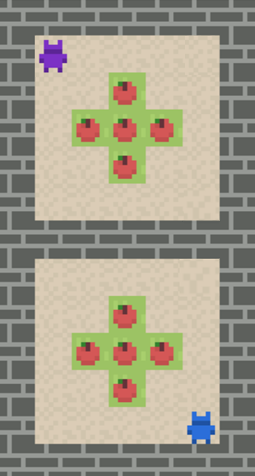
\includegraphics[width=.3\linewidth]{./figures/environments/train_priv.png}
  % \caption{Private property design}
  % \label{fig:train-env-priv}
  \centering
    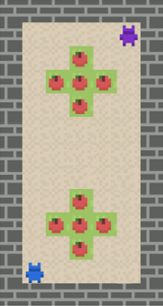
\includegraphics[width=.3\linewidth]{./figures/environments/train_collective.png}
  \centering
  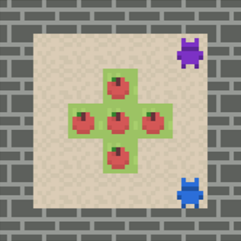
\includegraphics[width=.3\linewidth]{./figures/environments/evalulation.png}
  \centering
  \caption{In order: private property environment; collective property design; evaluation environment with the tragedy of the commons setting}
  \label{fig:envs}
\end{figure}  




\section{Experiments}
\subsection{Simulations}

The data sources of this study are in fact simulations in which trained agents are evaluated in pairs in the evaluation environment. This is a common practice in MARL research with environments implemented in the form of video games as in the utilized Melting Pot framework \citep{Leibo2021, agapiou2023meltingpot20}. Both the train and evaluation environment simulations last for 500 steps, thereby giving the time for agents to show with their behaviour whether they are able to cooperate with each other. Agents are trained for $10$ thousand episodes separately in respective environments, which translates to $5$ million steps. For the sake of gathering more robust results training both on collective and private environments utilized $5$ seeds each. 
% As a result of the fact that in each environment there are two agents, every training process resulted in two trained agents. Even though agents learn and interact with one another they can learn slightly different policies. With the aim of reducing bias, both agents from each training session for each seed were evaluated in the evaluation environment. 
In alignment with the intention of gathering broad results, trained agents were evaluated in pairs in distinct combinations: collective against collective, private against private -- and mixed: collective against private, and private against collective. As mentioned above, the spawn points of agents were randomised, regardless of the training environment. In total $10$ thousand simulations were run and agent scores were collected for statistical analysis of the impact of external motivators on co-operative behaviour. Wilcoxon signed-rank test \citep{Wilcoxon1945}, Two-sample paired sign test \citep{mendenhall1989nonparametric}, Mann-Whitney U test \citep{Mann1947}, and Brunner Munzel test \citep{Brunner2000}, along with necessary distribution diagnosis checks such as Shapiro-Wilk test \citep{Shapiro1965} and Levene test \citep{levene1960}, were used for statistical reasoning about the effects of different training environments with significance level $\alpha=5\%$. 
\subsection{Architecture}
The actor-critic model has been implemented, while the Proximal Policy Optimization (PPO) algorithm was used for training MARL agents, for details of this family of methods see \cite{Schulman2017}. The agent's architecture incorporates a Convolutional Neural Network with two layers of $16$ and $32$ output channels, with kernels of size $3\times3$ and $7\times7$ and stride equal to $1$ correspondingly. The graphical input for the PPO is downsampled to $7\times7$ pixels with dominant colours, which reduces the noise created by sprites and the $8$-bit aesthetic of the game. The outputs are connected to a fully connected Multi-Layer Perceptron with two layers of $64$ neurons each with ReLu activation functions. It is followed by a Long Short-Term Memory network with 128 cells. At the end, the policy of the actor and the value function of the critic are generated by linear layers. The discount factor $\gamma$ was set to $0.99$, the learning rate was set to $5\mathrm{e}{-4}$ and the entropy coefficient, which tunes the explore to exploit ratio was set to $0.01$. The SGD mini-batch size was $128$ and the number of SGD iterations was equal to $10$. Each agent learning period lasts for 5 million steps.

\subsection{Results}

After training agents separately in two distinct training environments, with the implementation of private property and collective property, they were examined in the evaluation environment. Agents were faced with the challenge of maximizing their expected total discounted reward which was equivalent to participating in long-term co-operation with the opposing party. Every agent was faced with one trained in the same environment or the alternative training environment as well as with copies of themselves. Noteworthy here is that each training session yielded two separate versions of agents. Agents were compared within the scope of the same seed, which translates to five separate experiments that after aggregation gave the final results. For the remainder of this study, a few terms will be referred to as follows.
% An agent trained in the collective property training environment will be referred to as a collective agent or CAgent for short. In the same manner, an agent trained in the private property training environment will be referred to as a private agent or PAgent for short. 
Four distinct evaluation scenarios can be distinguished: collective against collective (CC); collective against private (CP); private against collective (PC); private against private (PP). One can notice that the CP and PC scenario should be equivalent which is tested further.

\subsubsection{Homogeneous motivators}


In this subsection, the results of likely trained agents are compared -- namely, the CC and PP scenarios. The differences in behaviour between these two populations can be explored using the score distributions. All agent scores from both evaluation scenarios have been portrayed on the violin plots in Figure~\ref{fig:2-violin-CC-PP}. The distributions are similar in shape -- both are bimodal, however, the distribution of the CC scenario agent scores seems to be skewed towards higher values. This observation has to be examined with the use of appropriate statistical tools. The observations are independent as there is no interplay between the scenarios.

\begin{figure}[h!] 
  \centering
  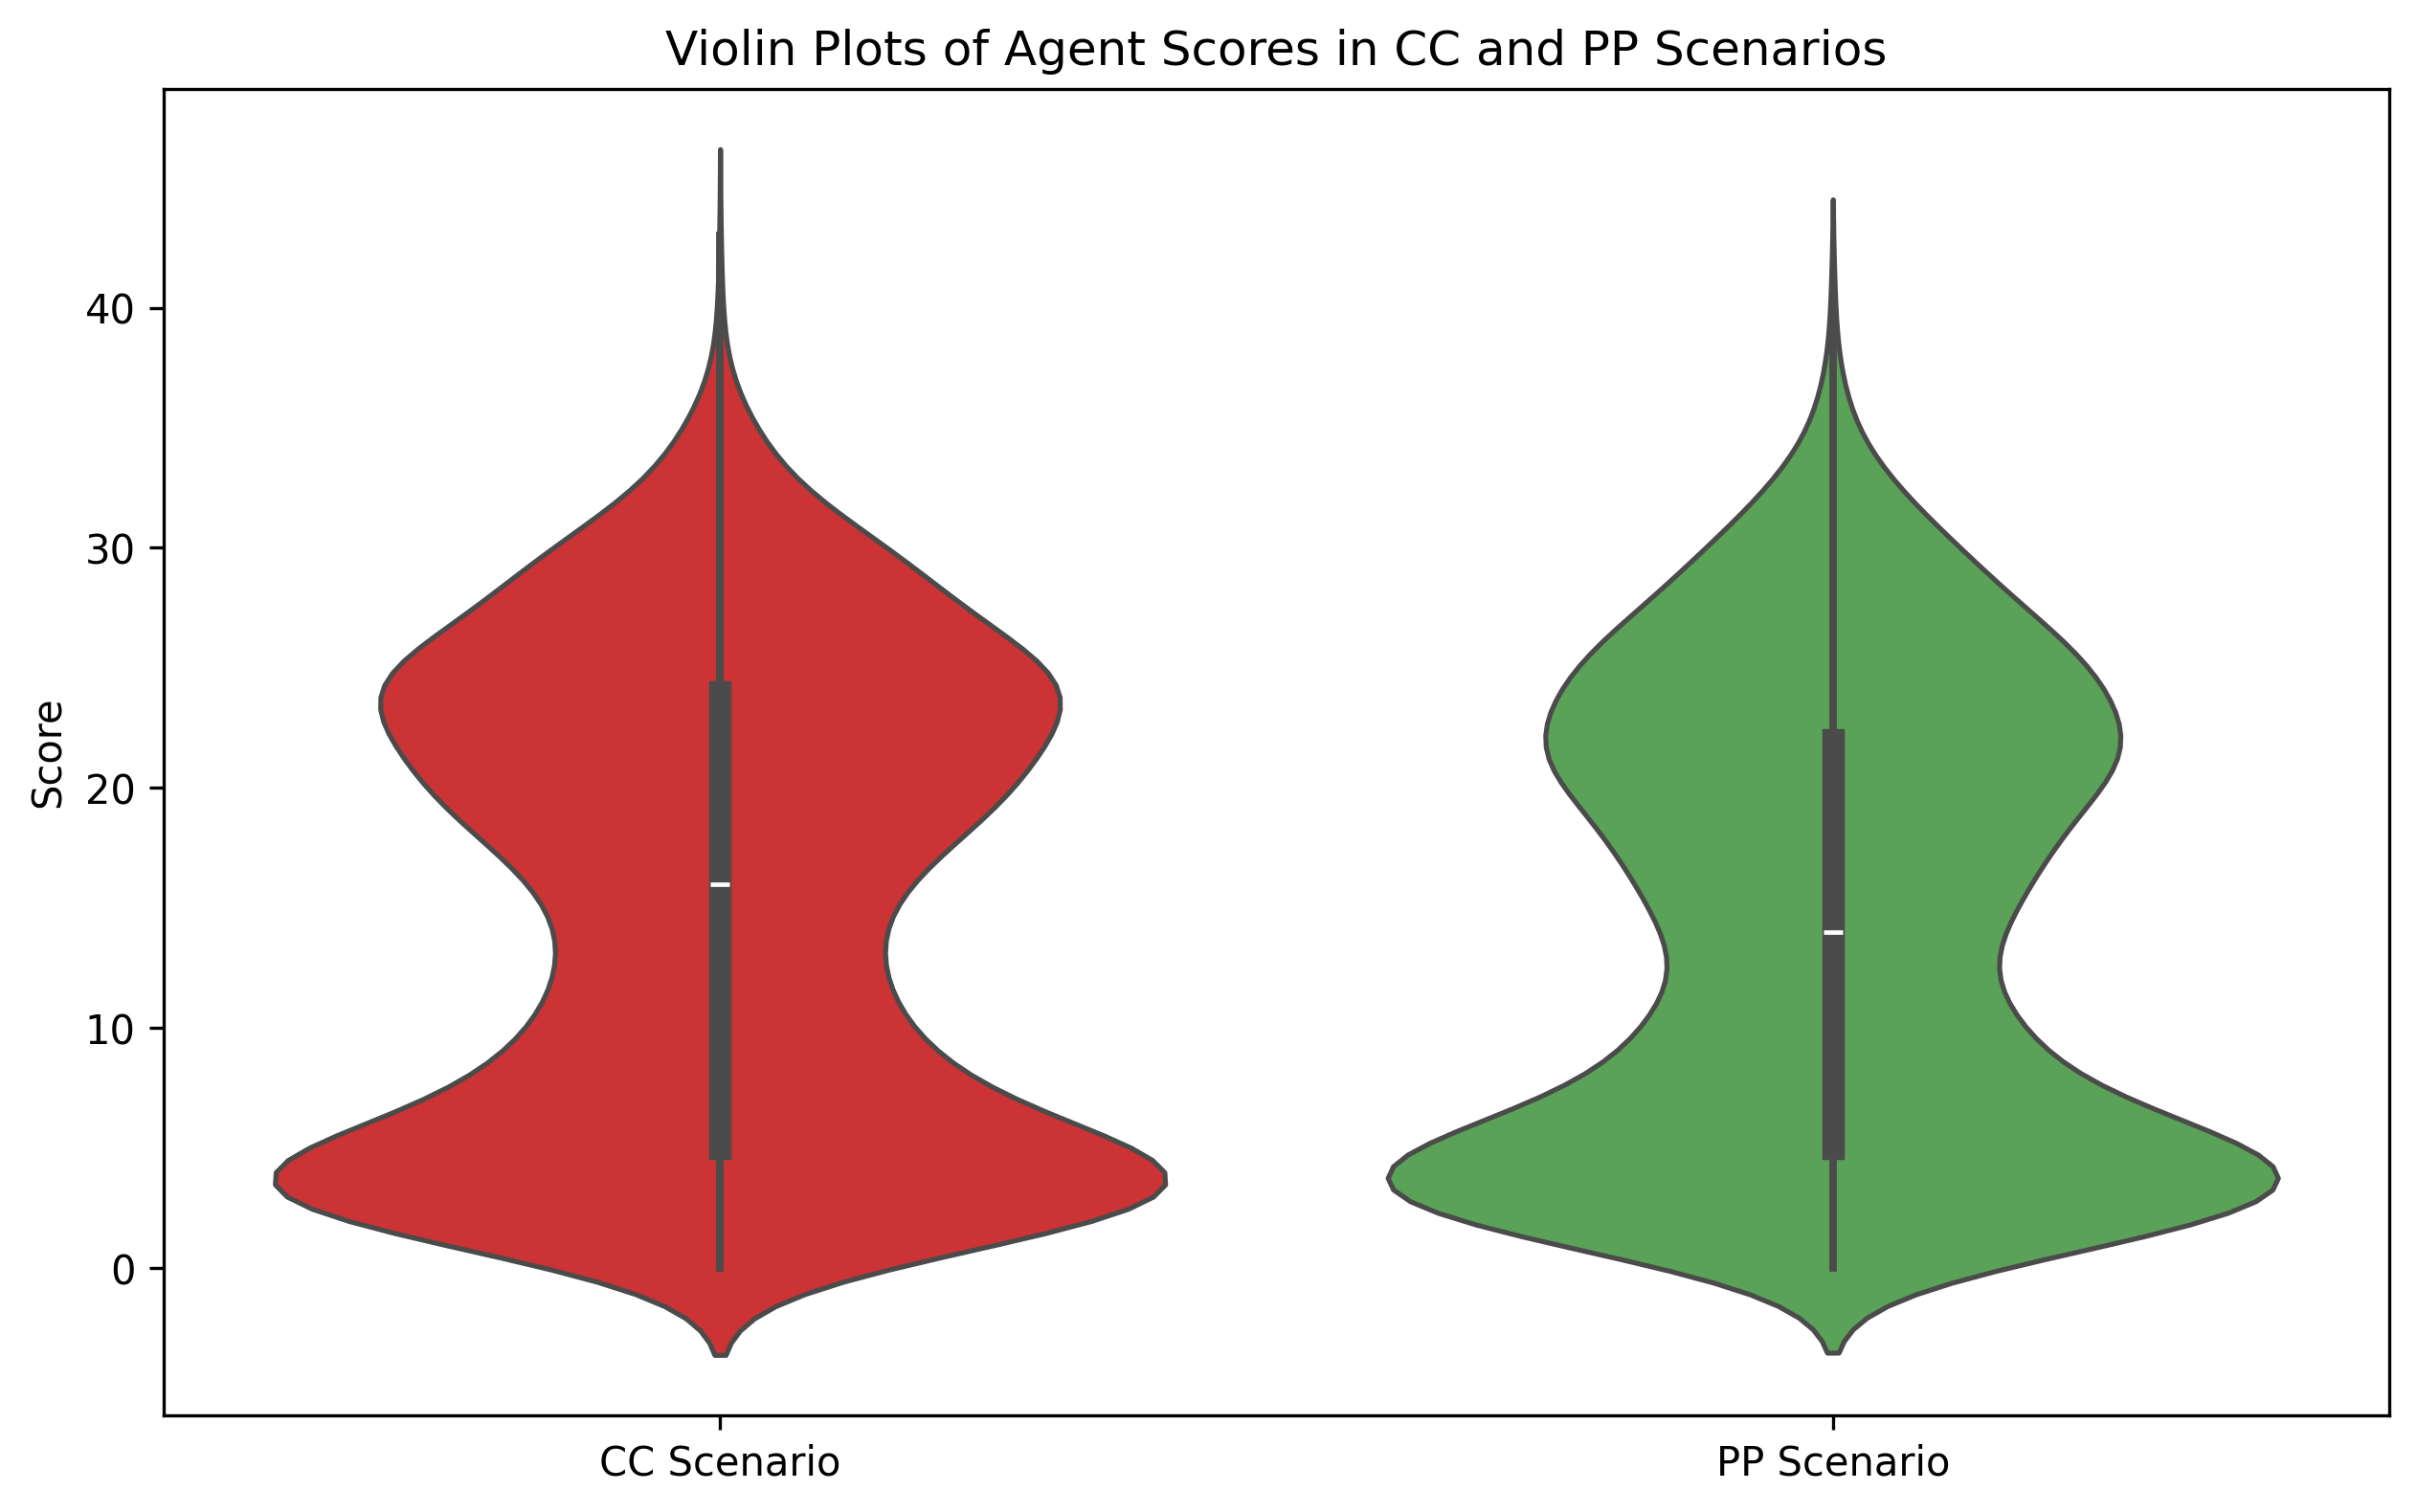
\includegraphics[width = .9\textwidth]{./figures/2_score_comparison/CC_PP_violin.png}
  \caption{Violin plots of the distribution of the agent scores in the CC evaluation scenario and the PP evaluation scenario.}
  \label{fig:2-violin-CC-PP}
\end{figure}  

In order to determine whether, in fact, the CC scenario has on average higher scores than the PP scenario, a battery of statistical tests was performed. Firstly, the normality of the distributions has been tested with the Shapiro-Wilk test. The null hypothesis about the normality of the distribution has been rejected for both samples with the corresponding p-values lower than the significance level $\alpha$, see Table~\ref{table:score-homo}. Secondly, the agent scores of both evaluation scenarios have been tested for homoskedasticity, as it is one of the assumptions of the Mann-Whitney U test. The Levene test for equal variances was computed for the CC and PP scenarios, which yielded a p-value lower than the significance level $\alpha$ (see Table~\ref{table:score-homo}). This resulted in the rejection of the null hypothesis about the equality of variances of both agent score samples. Given that the homoskedasticity assumption of the Mann-Whitney U test has not been met the alternative Brunner Munzel test has been computed. The null hypothesis of this test is compared against the one-sided alternative hypothesis 
% which states that for randomly selected values $X$ from the CC scenario and $Y$ from the PP scenario, the probability of $X$ being greater than $Y$ is greater than the probability of $Y$ being greater than $X$. 
% This would mean that 
which in analysed setting translates to collective agents having on average higher scores than the scores of private agents. 
% The Brunner Munzel test was applied and 
Resulting p-value was smaller than the significance level $\alpha$, which led to the rejection of the null hypothesis in favour of the one-sided alternative (see Table~\ref{table:score-homo}). 

\begin{table}[h!]
% \begin{adjustwidth}{-0.05\textwidth}{-0.05\textwidth}
\begin{tabularx}{\textwidth}{ccccc}
\toprule
Sample 1      & Sample 2      & Test                        & Statistic & p-value   \\ \midrule
Agents in CC &               & Shapiro-Wilk^r            & 0.93      & \textbf{4.5e-43}   \\
Agents in PP &               & Shapiro-Wilk^r            & 0.93      & \textbf{3.0e-43}   \\
Agents in CC & Agents in PP & Levene^r                   & 7.489     & \textbf{0.01}       \\
Agents in CC & Agents in PP & Brunner Munzel^g          & -4.63     & \textbf{1.8e-6}   \\ \bottomrule
\end{tabularx}

\caption{Results of statistical tests concerning the comparison of scores in the CC scenario and the PP scenario, significance level $\alpha=5\%$. r -- regular version of the test; g -- greater version of the test}
\label{table:score-homo}
% \end{adjustwidth}
\end{table}


% ------------------------------ dodane
In a general sense, the rejection of the null hypothesis in favour of the one-sided alternative means that on average collective agents (CAgents) in the CC scenario perform better than private agents (PAgents) in the PP scenario. Indeed the score distribution of the evaluations with two agents trained in the collective property training environment is shifted upwards compared to the score distribution of the evaluations with two agents trained in the private property training environment. In socio-economic terms, this suggests that the CAgents, when faced with like-minded individuals cooperate more often than PAgents in analogous settings. With the intention of holistic interpretation, we need to take into account both the apparent distributions from Figure~\ref{fig:2-violin-CC-PP}. and the results of statistical tests. From this information, we can deduce that the behaviour patterns of both the CAgents and the PAgents could be similar, however the former are capable of co-operating more often, hence the similarity of the shape of the distributions and statistically higher results in the CC scenario than in the PP scenario.

\subsubsection{Heterogeneous motivators}

The following paragraphs cover the comparison of the results of alternatively trained agents -- the collective agents faced against the private agents. As shown in the previous section the evaluation data points from the CP and PC scenarios can be combined into one dataset. The differences in behaviour between the CAgent and the PAgent populations can be explored using the score distributions. All agent scores from both evaluation scenarios have been portrayed on the violin plots in Figure~\ref{fig:2-violin-CA-PA}. The distributions are similar in shape -- both are bimodal, however, the distribution of the CAgent seems to be skewed towards higher values. This observation has to be examined with the use of appropriate statistical tools. The observations are dependent as there is direct interaction between the collective agents and the private agents.

\begin{figure}[h!] 
  \centering
  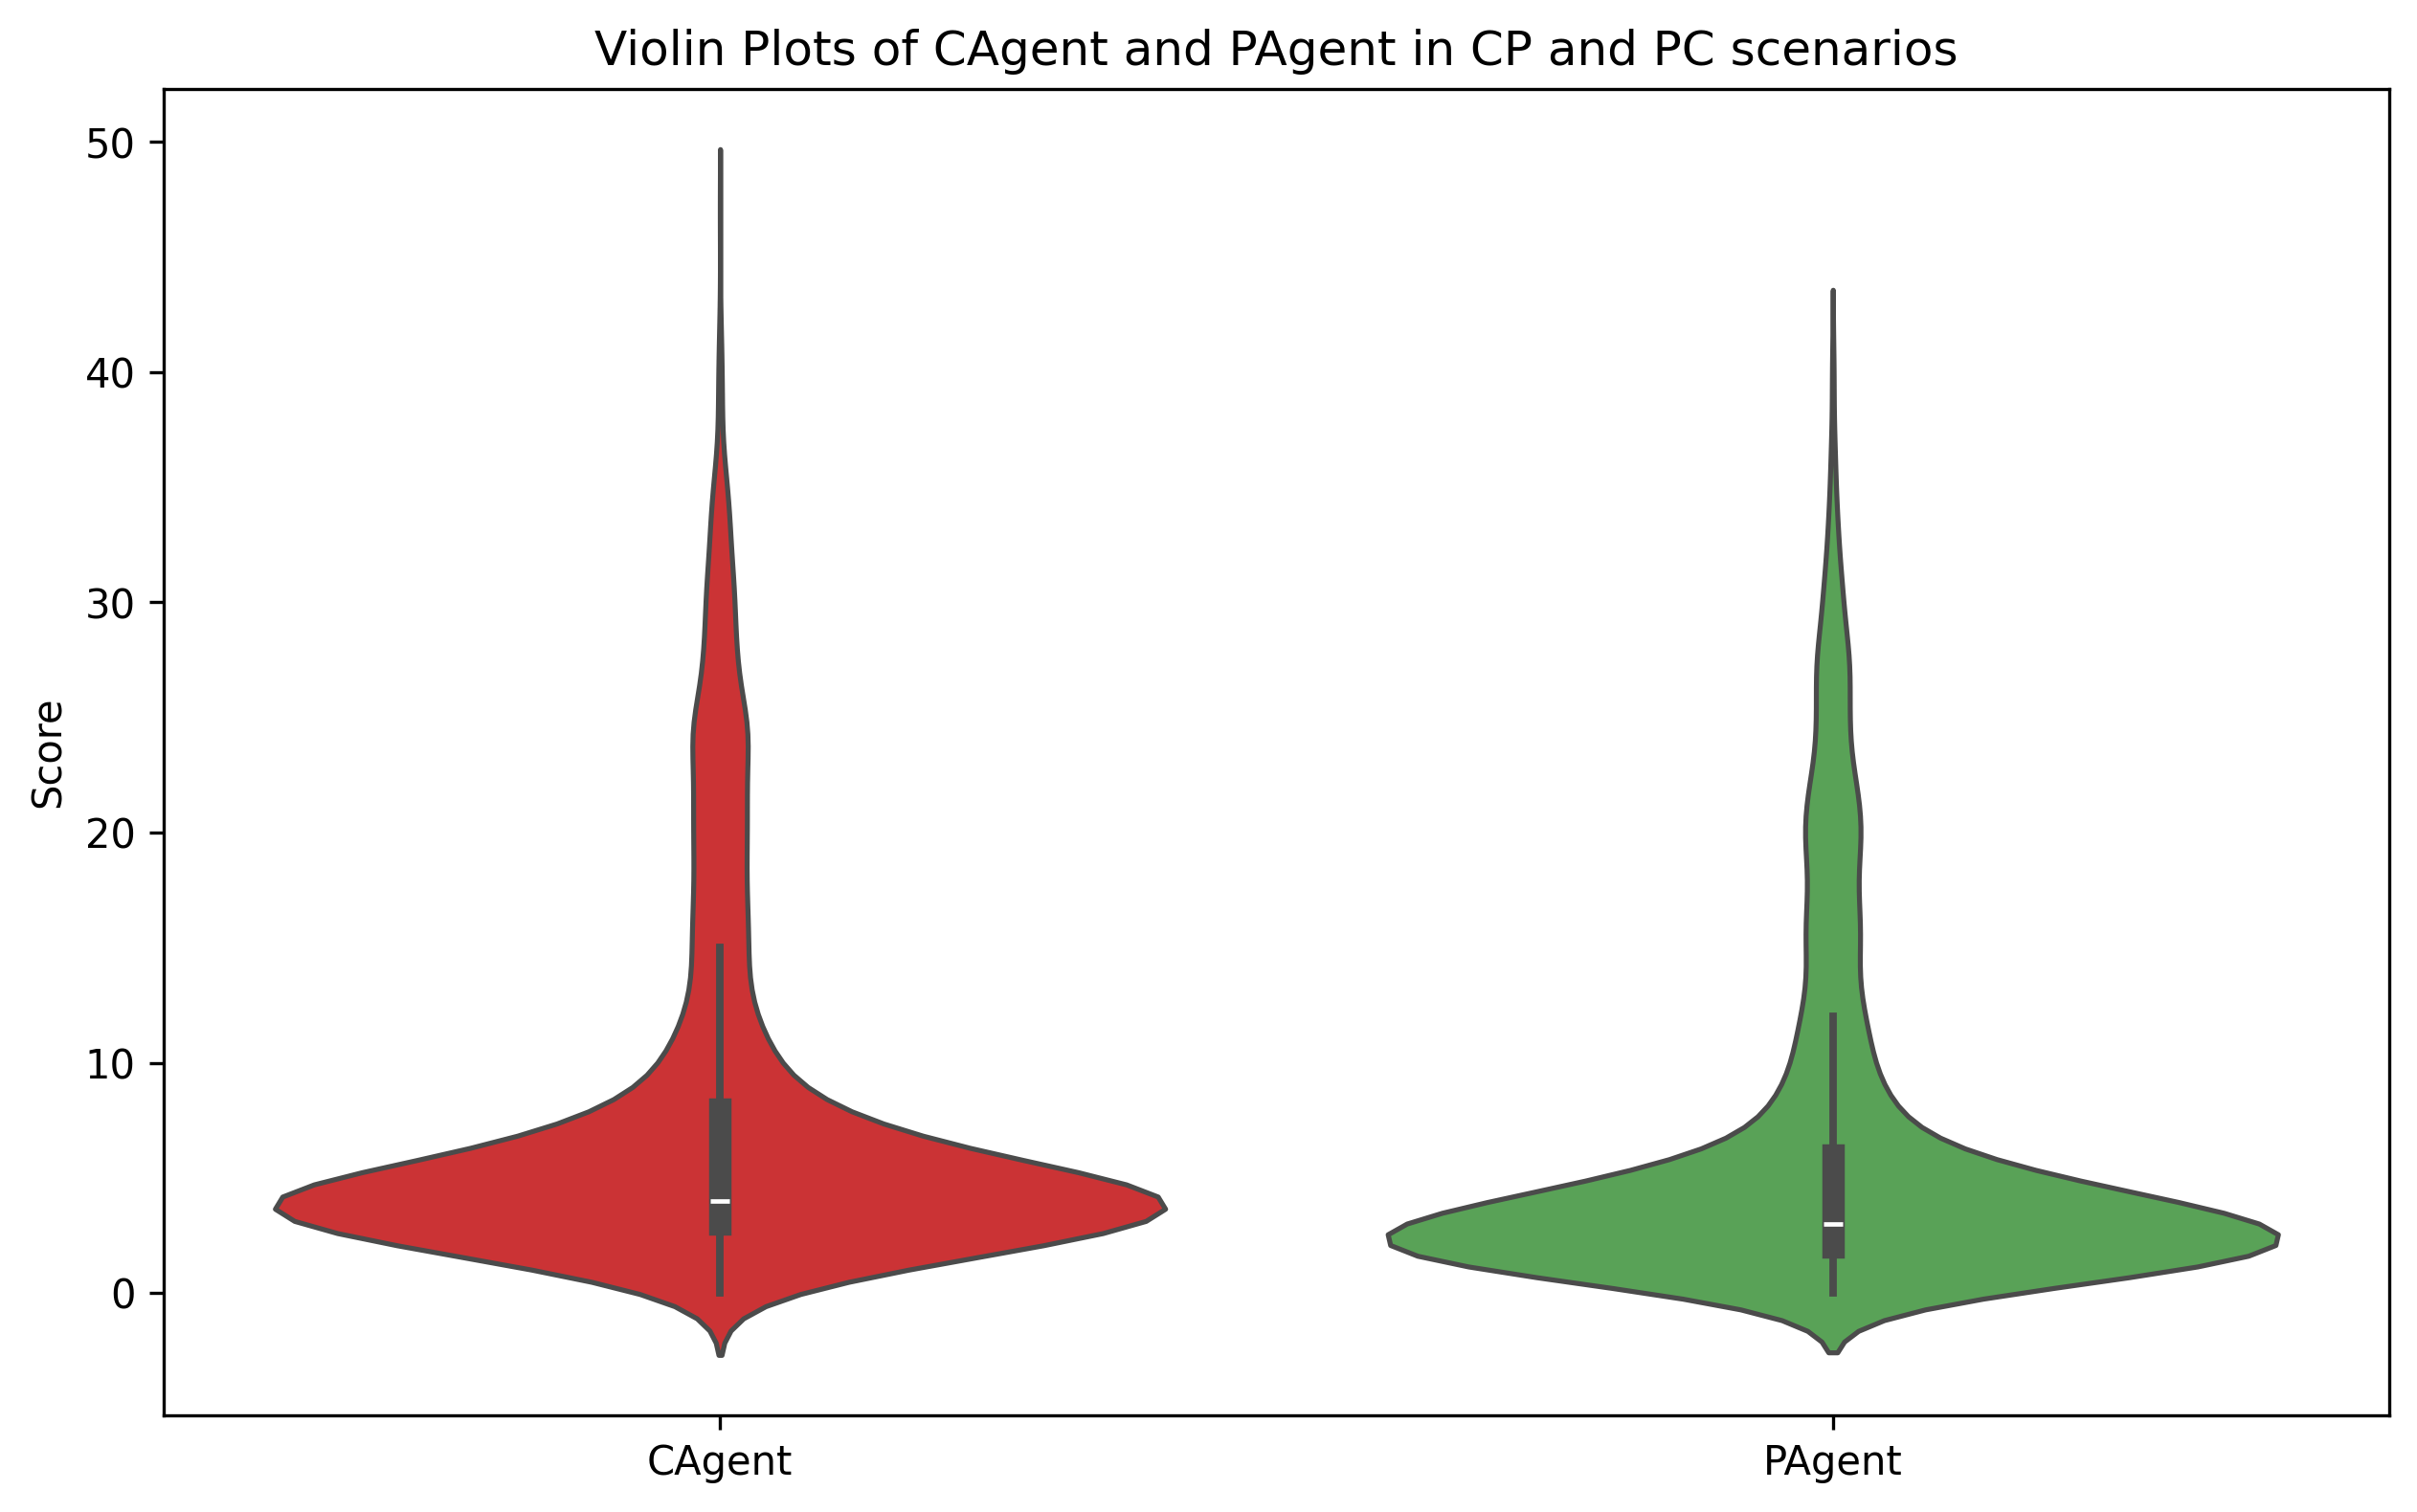
\includegraphics[width = .9\textwidth]{./figures/2_score_comparison/CAgent_PAgent_violin.png}
  \caption{Violin plots of the scores of the collective agents and the private agents in the CP and PC scenarios.}
  \label{fig:2-violin-CA-PA}
\end{figure}

In order to determine if the collective agents have on average higher scores than the private agents, a set of statistical tests was computed. Firstly, the normality of the distributions has been tested with the Shapiro-Wilk test. The null hypothesis about the normality of the distribution has been rejected for both samples with the corresponding p-values lower than the significance level $\alpha$, see Table~\ref{table:score-hetero}. Next, the distribution of differences between paired observations has been tested for symmetry, which is one of the assumptions of the Wilcoxon signed-rank test. The distribution of the differences has been investigated based on the density plots that reflect possible symmetry (see Figure A.6.). The skewness was also taken into account, which was equal to $0.36$ and this alludes to symmetry, given that the value is near $0$. Lastly, mean and median were compared, as close values of said descriptive statistic imply symmetry of the underlying distribution i.e., the values were $1.31$ and $1$ respectively. Since the assumptions of the Wilcoxon signed-rank test are most likely met, the one-sided version was used to test whether the distributions of scores of the collective agent and the private agent differ. The alternative hypothesis 
% states that the median of the distribution differences of scores between the collective agent and the private agent is greater than $0$, 
translates to collective agents on average performing better than the private agents. The null hypothesis was rejected in favour of the one-sided alternative, as the p-value was smaller than the significance level $\alpha$ (see Table~\ref{table:score-hetero}). To ensure the robustness of the previous test, the alternative test for distributions without symmetrical differences -- the two-sample paired sign test has been performed. The results are in line with the Wilcoxon signed-rank test, as shown in Table~\ref{table:score-hetero}.

\begin{table}[h!]
% \begin{adjustwidth}{-0.1\textwidth}{-0.1\textwidth}
\begin{tabularx}{\textwidth}{ccccc}
\toprule
Sample 1             & Sample 2             & Test                        & Statistic & p-value   \\ \midrule
CA in CP/PC &                      & Shapiro-Wilk^r            & 0.71      & \textbf{1.9e-68}    \\
PA in CP/PC &                      & Shapiro-Wilk^r            & 0.70      & \textbf{1.3e-69}    \\
CA in CP/PC & PA in CP/PC & signed-rank^g    & 7.3e6     &  \textbf{3.3e-105}  \\
CA in CP/PC & PA in CP/PC & paired sign^g  & 732     &  \textbf{1.8e-104}  \\ \bottomrule
\end{tabularx}
\caption{Results of statistical tests concerning the comparison of scores of the collective agents and the private agents, significance level $\alpha=5\%$. r -- regular version of the test; g -- greater version of the test; CA -- collective agent, PA -- private agent}
\label{table:score-hetero}
% \end{adjustwidth}
\end{table}


The interpretation of the aforementioned results is rather counter-intuitive. The agents trained in a collective property environment outperform those trained in a private property environment while being in direct confrontation with one another. One would assume that the PAgents would often rush for the apples and as a result leave no reward for the CAgents. However, the collective agents do not simply look at the apples being eaten, they also harvest them. In fact, they behave in such a way that gives, on average, an edge over the private agents. As the median score is around $5$ for both agents, this shows that even if co-operation exists, it lasts breifly. Two valuable insights can be drawn from these findings about the behaviour of both agent types. Firstly, the CAgents can take more from even a short-lasting co-operation, this is probably due to maximal feasible harvesting at the beginning of the evaluation which leaves one apple in the patch and is a kind of an invitation to co-operate. Secondly, the PAgents can in fact cooperate, which is shown by the tails of the distributions however, they tend to hamper co-operation from being long-lasting. Moreover, strong co-operation between agents is less frequent than in the homogeneous CC and PP scenarios which is indicated by the scores being skewed towards lower values.

\subsection{Behaviour analysis}

For the purpose of a more in-depth analysis of the behaviour of the agents, videos of their interactions have been rendered and analyzed. Videos covered all of the possible evaluation cases: CC, CP, CP and PP scenarios. It is worth noting that only a fraction of the results could be verified with video analysis since there were $10$ thousand simulations run during the evaluation. 
% In general, patterns that were found in the statistical analysis of the results in previous subsections can be observed in the videos that are examined in this subsection. These videos are available in the project repository. 

Firstly, the example of long-lasting co-operation i.e., both agents harvesting apples responsibly by leaving at least one apple in the patch at all times, is showcased. This behaviour was mostly observed in the CC evaluation scenario, as in the CC-25-23 video. The final score of this specific evaluation was $25$ to $23$ with both agents co-operating seamlessly. 
% However, there is not always long-lasting co-operation even between two collective agents.  
A good illustration of short-lasting co-operation can be found in the CC-8-8 video where one of the agents suddenly eats the last apple. The final score is uniform among the agents with scores of $8$ and $8$ at the end of the evaluation episode. This behaviour is suspected to be a consequence of the length of the training period and is thought to be removed given longer training windows -- answering this question is open for further research. 
% Nevertheless, the egalitarian score distribution highlights the co-operation and sharing of resources between both collective agents.

Secondly, cases of selfish behaviour can be highlighted, i.e., eating the last apple left in the patch to gain a short-term reward of $1$ and disabling regrowth.
% but at the same time removing the possibility of earning higher rewards for both agents in the remainder of the evaluation episode. 
Such instances can be found in the PP evaluation scenario like in the PP-14-9 video. Domination of one of the agents can be seen during the evaluation episode, where one of the agents harvests most apples for themselves while the other agent harvests only several apples. This evaluation finished with scores of $14$ and $9$ respectively
% , where the more dominant agent eats the last apple at some point. 
This video is an instance of short-lasting co-operation with the interaction between two private agents yielding uneven scores, while the harvesting episode is finished prematurely.


Lastly, the CP and PC evaluation scenarios were examined based on generated videos. One could notice that the agent score distributions vary between the CC and PP scenarios compared to the score distributions of the CP and PC scenarios, see Figure~\ref{fig:2-violin-CC-CP-PC-PP}. The score distributions from homogeneous motivators scenarios are bimodal with peaks around scores of $5$ and $25$ for both agents. The lower one corresponds to short-lasting co-operation with only a few apples regrowing, while the higher one corresponds to long-lasting co-operation with multiple episodes with only one apple present, i.e., enough to regrow more apples while harvesting the rest. On the other hand, the score distribution from heterogenous motivators scenarios is unimodal with one peak around the score of $5$ for both agent types. This shows that mostly the cooperation of CAgent and PAgents was short-lasting, however, the tail of high scores shows that these agent pairings can in fact co-operate in longer time frames. 


\begin{figure}[h!] 
  \centering
  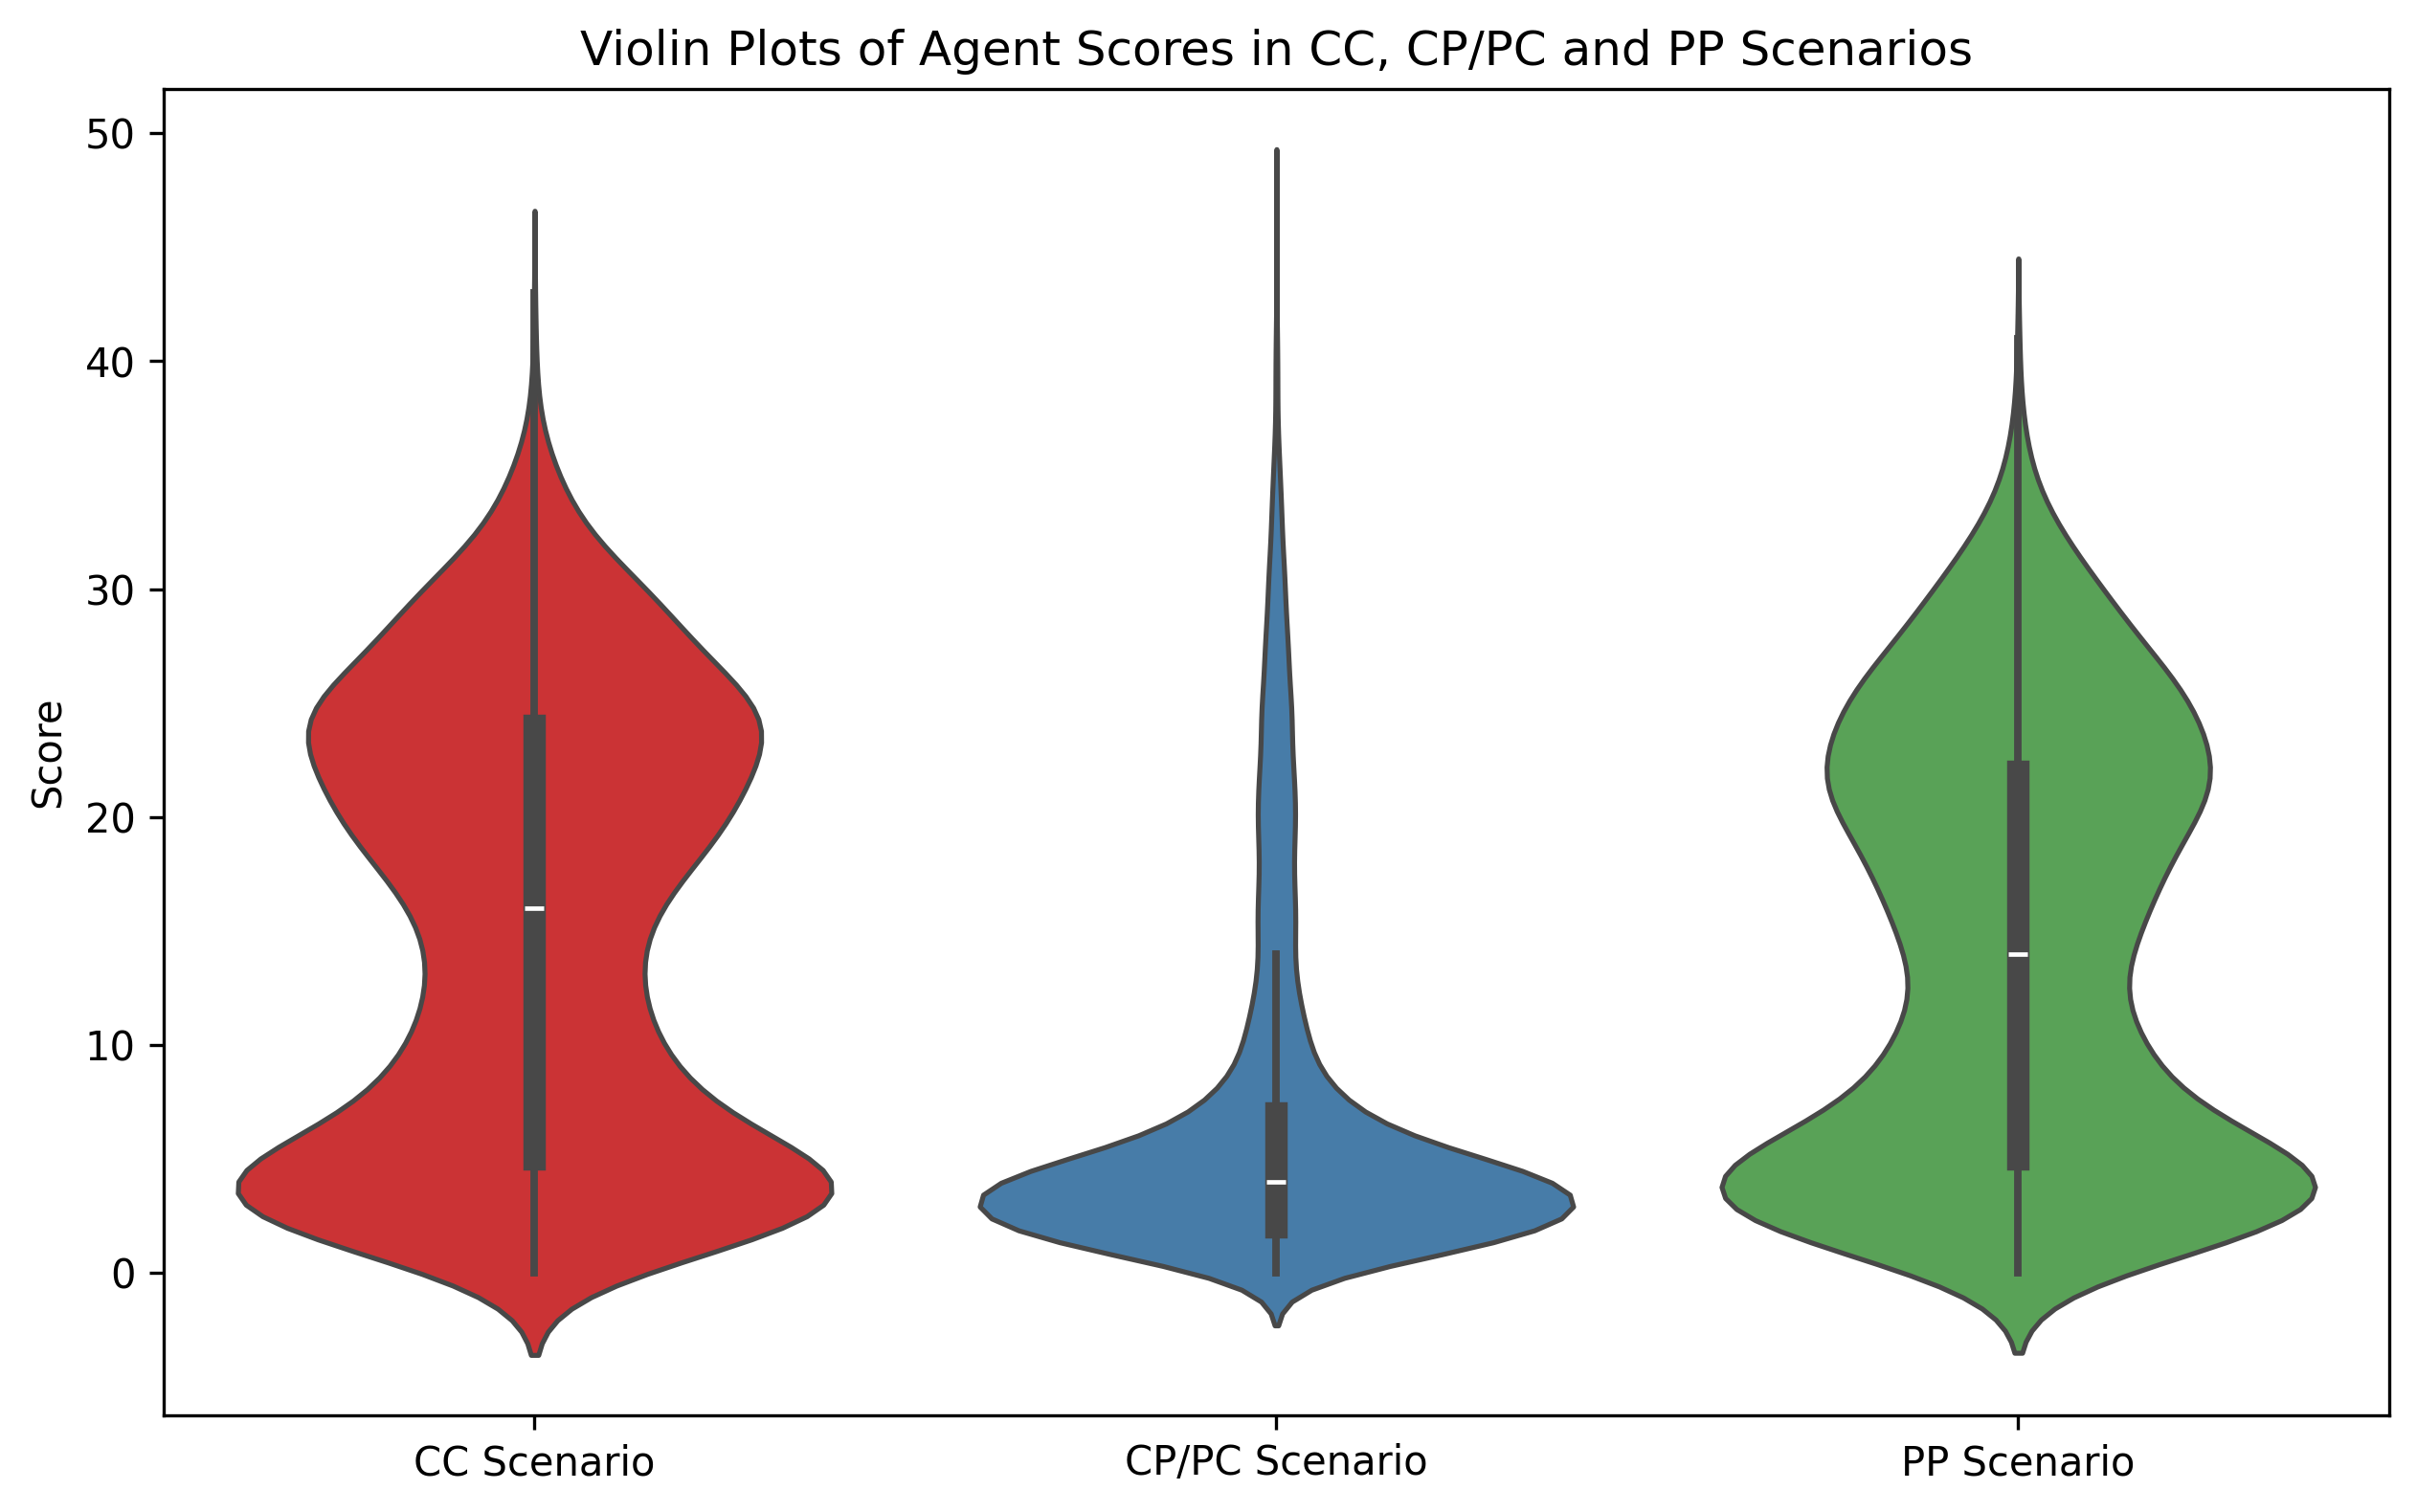
\includegraphics[width = .9\textwidth]{./figures/2_score_comparison/CC_CP_PC_PP_violin.png}
  \caption{Comparison of the violin plots of the distributions of agent scores in the CC, CP/PC and PP evaluation scenarios, own work.}
  \label{fig:2-violin-CC-CP-PC-PP}
\end{figure}  


The substantial dissimilarity between homogeneous and heterogeneous motivators score distributions is possibly due to a larger difference in behaviour between playing with like-minded agents and opposingly trained agents. The change in the environment is greater and such behaviours likely have not been encountered during the training period, resulting in a drop in performance. We suppose that these discrepancies could be lowered by extending the learning periods in the training environments. The PC-2-4 video shows the private agent acting selfishly relatively early in the evaluation episode, resulting in both agents having low scores. In this specific case, it was $2$ and $4$ respectively. However, it is not as trivial as the private agents always being the ones to eat the last apple in the patch in every simulation. There are examples, such as the video CP-2-4, where the collective agent is the one responsible for depleting the patch of apples prematurely, which results in final scores of $2$ and $4$ respectively.



% In summary, co-operation behaviour has been found among both the CC scenario and the PP scenario, however, it is more common among agents that were trained in the collective right property environments. Conversely, it is more frequent among the agents that were trained in the private property rights environments to behave selfishly and refuse to co-operate. The pairings of collective agents with private agents perform worse relative to the other evaluation scenarios, and this is likely caused by the bigger difference in the evaluation environment compared to the training environment. Altogether, the policies which lead to co-operation are harder to develop by the agents as they are on a higher level of abstraction and necessitate looking forward in time. 

% Given the results of the statistical tests comparing populations in distinct evaluation scenarios and evidence derived from the videos of agents’ behaviour, the stated hypotheses can be verified. 
The analysis of the results highlights that both the CC evaluation scenario and the PP evaluation scenario had long-lasting co-operation occurring. This shows that both collective agents and private agents can co-operate
% : however, the statistical analysis of the scores and rendered interaction videos suggest that the former are more capable of co-operation than the latter. 
The collective agents in the CC scenario were more likely to score more than private agents in the PP scenario, thus making the co-operation last longer. The tendency of private agents to break co-operation has been observed in the rendered videos. Based on these premises the first hypothesis can be verified positively. The “well-being” of agents in the Commons Harvest setting can be understood as the final aggregated reward, which might be seen as a pseudo-utility function. The statistical analysis of the scores in all evaluation scenarios shows that collective agents score, on average, more than the private collective agents, regardless of the scenario being homogeneous or heterogeneous. Consequently, the second hypothesis can be verified positively. In the case of the third hypothesis, the conclusions are more nuanced. On the one hand, the behaviour and the interactions of two collective agents in the CC scenario are more co-operation-oriented and yield better “well-being” than the CP and PC scenarios. This would suggest that for a collective agent, it would be beneficial to replace a private agent with another collective agent. On the other hand, the agents in the CP and PC scenarios have on average lower “well-being” than the agents in the PP scenario. This would indicate that for a private agent, it would be detrimental to replace another private agent with a collective agent. From these premises we can deduce that it is not always beneficial to replace a private agent with a collective agent, however, it indicates that there might be a critical mass point where after adding enough collective agents the “well-being” will increase. Taking into account these findings, the third hypothesis can be verified negatively.

\section{Conclusion}


This article investigates the influence of external motivators, in the form of property rights, on ensuring co-operative behaviour in Multi-agent Reinforcement Learning (MARL) agents within a tragedy of the commons socio-economic setting. The focus was placed on the modification of the Commons Harvest environment, which is a part of the Melting Pot library \citep{Leibo2021, agapiou2023meltingpot20}. An agent's self-interest can lead to the depletion of shared resources, whereas co-operation allows for higher final scores, mirroring real-world situations like overfishing or deforestation.


Three hypotheses are tested, the first one states that agents trained in the environment with collective property rights, where resources are shared and managed collectively, would be more prone toward co-operation than agents trained in environments with private property rights, where resources are individually owned and controlled. The second hypothesis states that agents trained in collective property environments will achieve higher scores than those trained in private property environments. The third hypothesis states that the inclusion of collective agents into a population will increase the score.

These results provide statistically significant evidence supporting the two first hypotheses. However, the third hypothesis is falsified. The agents trained in collective property environments demonstrate significantly higher levels of co-operation and achieve higher scores than those trained in private property environments. What is more, the collective agents have higher scores regardless of playing against the collective agents of private agents. Lastly, the inclusion of a collective agent does not necessarily lead to a rise in the scores of the population. This suggests that external motivators, such as the implementation of property rights, can significantly influence the emergence of co-operative behaviours in MARL agents.


Furthermore, analysis of the videos rendered, based on the evaluation scenarios, confirms the suspected behaviours of agents in different scenarios. The collective agents are more likely to co-operate, leaving some apples for regrowth, leading to long-term sustainability. Conversely, private agents display more selfish behaviour, often depleting the resources for short-term gains, ultimately leading to poorer long-term outcomes for everyone involved. 
% Agents trained in environments with contrasting external motivators exhibit different behavioural patterns, indicating that the environment's design plays a role in shaping the final policy.

This article contributes valuable insights into the design and implementation of MARL agents in real-world-like scenarios, particularly those involving resource management requiring co-operation. It emphasizes the potential of external motivators, like property rights, in promoting co-operative behaviour and achieving sustainable outcomes. Further research could study the co-operation in larger, more complex, populations of four or more agents as well as effect of resource scarcity. 
% -- i.e., different spawning rates of apples on the emerging behaviour. 
The interplay between external and internal motivators could be researched, for instance by implementing reward transfer on top of the property rights implementation. There is still a lot to be done to understand and optimize the co-operative behaviour of agents.

%%%%%%%%%%%%%%%%%%%%%%%%%%%%%%%%%%%%%%%%%%%%%%%%%%%%%%%%%%%%%%%%%%%%%%%%

\vspace{10pt}

\textit{This research did not receive any specific grant from funding agencies in the public, commercial, or not-for-profit sectors.}

% \bibliographystyle{elsarticle-num}
\bibliographystyle{unsrt}
\bibliography{bibliography.bib}

\end{document}


\endinput
%%
%% End of file `elsarticle-template-harv.tex'.


